\documentclass{standalone}
\usepackage{PhysicalChemistryNote}
\begin{document}
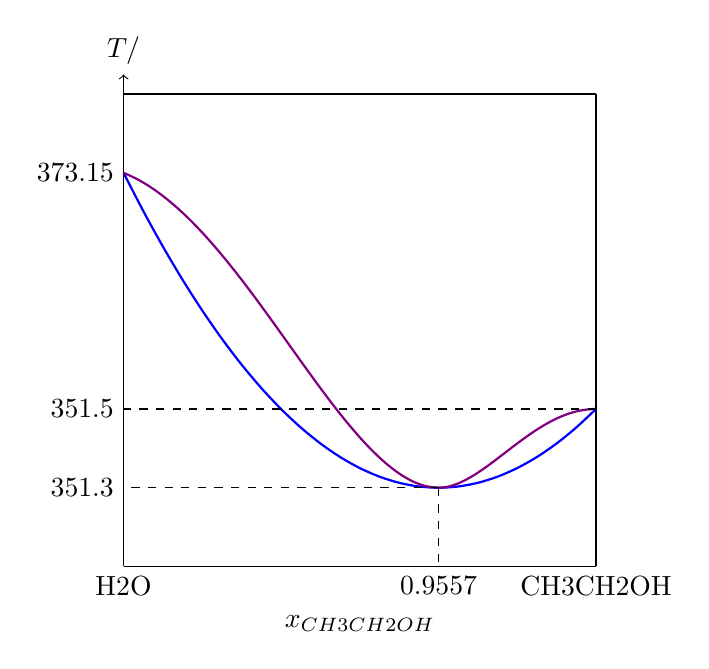
\begin{tikzpicture}
    \draw[-] (0,0) -- (6,0);
    \draw[->] (0,0) -- (0,6.25) node[above]{$T/\K$};
    \draw[-] (6,0) -- (6,6);
    \draw[-] (0,6) -- (6,6);
    \node[below] at (0,0) {{\ce{H2O}}};
    \node[below] at (6,0) {{\ce{CH3CH2OH}}};
    \node[below] at (3,-0.5) {$x_{\ce{CH3CH2OH}}$};
    \draw[domain=0:6,thick,blue] plot[smooth](\x,{(\x-4)^2/4+1});
    \draw[domain=0:4,thick,violet] plot[smooth](\x,{(\x+5)^2*(\x-4)^2/100+1});
    \draw[domain=4:6,thick,violet] plot[smooth](\x,{(\x-4)^2*(\x-8)^2/16+1});
    \draw[dashed] (4,1)--(4,0) node[below]{$0.9557$};
    \draw[dashed] (4,1)--(0,1) node[left]{$351.3\K$};
    \draw[dashed] (6,2)--(0,2) node[left]{$351.5\K$};
    \node[left] at (0,5) {$373.15\K$};
\end{tikzpicture}
\end{document}